\chapter{Huidige situatie}

\label{Chapter4}

Dit hoofdstuk gaat over de deelvraag \enquote{\deelhuidig}. Dit wordt beantwoord

\section{Huidige Architectuur}
De huidige website is een combinatie van een PHP \& Symfony back-end API en Content Management Systeem, samen met een React + next.js front-end. De infrastructuur is momenteel gebouwd op Docker(-compose) + Ansible. Bitbucket pipeline wordt gebruikt voor het Continuous Integration / Deployment. 

In figuur \ref{fig:infra} is een component diagram te vinden van de huidige website structuur. De front-en backend structuur bevat 5 docker containers:
\begin{itemize}
	\item \textbf{PHP-FPM} (back-end)
	\item \textbf{Nginx} (front-en backend)
	\item \textbf{Redis} (back-end)
	\item \textbf{NodeJS} (front-end)
	\item \textbf{PostgreSQL} (back-end)
\end{itemize}

\begin{figure}
	\centering
	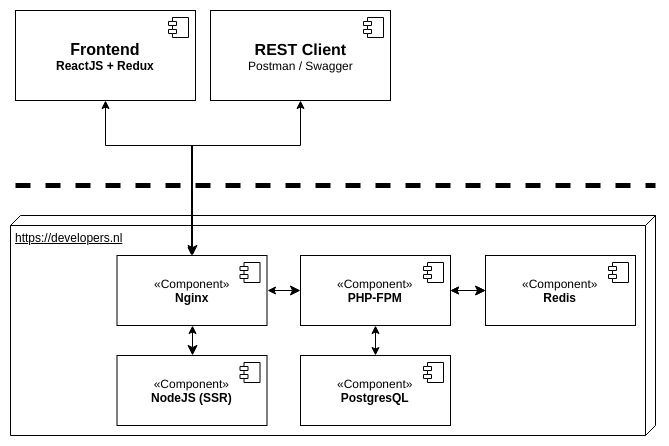
\includegraphics[width=13cm]{Figures/Infrastructure}
	\decoRule
	\caption[Infrastructuur]{Infrastructuur website front-en backend \parencite{Documentation}}
	\label{fig:infra}
\end{figure}

PHP-FPM is een FastCGI Process Manager, deze Container serveert de Symfony “FosREST” API en het Content Management Systeem. De NodeJS container serveert een statische Next.js React applicatie en maakt gebruik van Server Side Rendering. Er zit een Nginx reverse proxy in die kiest om een request naar de back-end of de front-end te laten gaan. Redis is een Key-Value Database die gebruikt wordt voor het cachen, en een PostgreSQL container als database. De Bitbucket Pipeline gebruikt Ansible om op de servers de geüpdatete containers te pullen en te starten.

Voor zowel de front- als backend is één monitoring tool genaamd \enquote{Sentry} geïmplementeerd. Sentry creëert een duidelijk overzicht voor alle errors die opkomen in productie.

Ook heeft Developers.nl een \enquote{Employee Management Systeem} (EMS) gebouwd. Deze heeft een soortgelijke structuur aan de website. Het EMS bevat zeer veel gevoelige informatie en het is dus van hoog belang dat deze goed beveiligd is.

\section{Metingen}

Nu de infrastructuur in kaart is gebracht luidt de vraag; hoe schaalbaar is deze infrastructuur eigenlijk? Om dit te beantwoorden worden de verschillende definities van schaalbaarheid individueel behandeld.

\subsection{Structural scalability}
Definitie: Het vermogen van een systeem om uit te breiden in een gekozen dimensie zonder ingrijpende wijzigingen in de architectuur.

Bij structural scalability horen factor 2 \textbf{(API First)} en 5 \textbf{(Configuration, credentials, and code)} van de 15-factor app. 

\subsubsection{API First}
De website van Developers.nl is momenteel in 2 delen gesplitst: de React Front-end en de PHP API als back-end. Deze worden apart ontwikkeld, waardoor dus het principe altijd wordt toegepast. Daarnaast heeft het EMS geen API, en is dus out-of-scope.

\subsubsection{Configuration}
Een test om te bewijzen dat alle configuratie correct uit de code is verwerkt, is of de applicatie op elk gewenst moment open-source kan worden gemaakt zonder geclassificeerde informatie vrij te geven.

Voor de website wordt er gebruik gemaakt van docker-secrets en ansible-vault. Deze combinatie zorgt ervoor dat er nooit wachtwoorden, API sleutels en dergelijke plain-text in versiebeheer komt te staan. Deze secrets worden uiteindelijk in de containers als environment variabelen opgeslagen en uitgelezen door Symfony. In het EMS is deze techniek nog niet gebruikt en staan credentials wél plaintext in de repository.

Om aan factor 5 te voldoen moet de configuratiefiles niet per specifieke omgeving (productie, test, staging) gegroepeerd worden maar moeten juist individueel per deployment geregeld worden. Dit gebeurt in zowel het EMS als de website, de bitbucket pipeline heeft zijn eigen specifieke environment variabelen om te gebruiken en de variabelen in de docker containers worden meegegeven in de algemene docker-compose file die in elke deployment hetzelfde zal zijn.

\subsection{Load scalability}
Definitie: Het vermogen van een systeem om elegant te presteren naarmate het aangeboden verkeer toeneemt. Om een load-test uit te voeren zijn meerdere tools met elkaar vergeleken:
\begin{itemize}
	\item https://loader.io/
	\item https://gatling.io/
	\item https://k6.io/
	\item http://tsung.erlang-projects.org/
\end{itemize}

De gratis versie van loader.io is niet genoeg voor de wensen van de test, voor gatling.io is Ruby kennis nodig, en voor Tsung worden de tests in XML geschreven wat het lastig maakt om de load op te schalen. Uiteindelijk is gekozen voor K6 omdat zo goed als elke ontwikkelaar genoeg Javascript kennis heeft om deze tool te gebruiken. Ook heeft k6 een gemakkelijke manier om de hoeveelheid Virtual Users (VU) geleidelijk te verhogen. Om de uitkomsten te visualiseren is InfluxDB samen met Grafana gebruikt. In bijlage \ref{Bijlagek6} is de implementatie hiervan te vinden.

Bij load scalability horen factor 12 \textbf{(stateless processes)}, 13 \textbf{(concurrency)} en 7 \textbf{(disposability)} van de 15-factor app methodologie. 

\subsubsection{Stateless processes}
Factor 12 vereist dat de applicatie als één of meerdere \enquote{stateless processes} moet uitgevoerd worden. Bij de PHP containers worden geüploade bestanden weggeschreven naar een volume, dit zorgt ervoor dat de container niet volledig stateless meer is. Ook zijn databases in docker containers geplaatst, dit is een stateful process aangezien het van belang is dat niet alle data verloren gaat zodra de container stopt.

\subsubsection{Concurrency}
Voor factor 13 is het van belang dat een applicatie horizontaal uit te schalen is. Zolang de applicatie aan factor 7 (Disposability) en 12 (Stateless processes) voldoet zit deze factor goed \parencite{Beyond12Factor}.

\subsubsection{Disposability}
Voor factor 7 moet een applicatie opstarttijd minimaliseren. Zodra de docker images de initiële buildtime voorbij zijn kan de applicatie snel uit en aan worden gezet. \textcolor{red}{TODO: HOE SNEL?} % TODO: Hoe snel?

Ook vereist factor 7 dat processen netjes worden afgesloten zodra ze een \texttt{SIGTERM} ontvangen. Zodra een docker container met \texttt{docker stop <container>} gestopt wordt zal er een SIGTERM worden gestuurd naar de draaiende processen. De vier containers met processen zijn PostgreSQL, PHP-FPM, Nginx en Redis. Deze sluiten allemaal netjes af, de outputs zijn te zien in Bijlage \ref{DockerExits}.

Ook moeten de processen bestendig zijn tegen \enquote{sudden death}. Om dit te simuleren kan \texttt{docker kill <container>} gebruikt worden om een \texttt{SIGKILL} te sturen naar de hoofdprocessen. In bijlage \ref{DockerKills} is te zien dat alle containers na een \texttt{docker kill} zonder problemen weer kunnen opstarten.

\subsubsection{Weinstock \& Goodenough controle}
Om de schaalbaarheid te waarborgen zullen de 3 methoden van Weinstock en Goodenough \parencite{OnSystemScalability} uitgevoerd worden:

\begin{itemize}
	\item Performance curves
	\item Knelpunten
	\item SWOT
\end{itemize}


\subsection{Functional scalability}
Definitie: In welke mate bestaande code moet worden aangepast zodra een nieuwe functionaliteit wordt toegevoegd aan het systeem.

Binnen de scope van de infrastructuur.

\subsection{Onderhoudbaarheid}
Definitie: The degree of effectiveness and efficiency with which a product or system can be modified to improve it, correct it or adapt it to changes in environment, and in requirements.

\section{conclusie}
